\section{Verified Deterministic Parallelism}\label{sec:eval-parallelism}

Finally, we evaluate our deterministic
parallelism prototypes.  Aside from the lines of proof code added,
we evaluate the impact on runtime performance.
%
Were we using a proof tool external to Haskell, this would not be necessary.
But our proofs are Haskell programs---they are necessarily visible to the
compiler.  In particular, this means a proliferation of unit values and functions
returning unit values.  Also, typeclass instances are witnessed at runtime by
``dictionary'' data structures passed between functions.  Layering proof methods
on top of existing classes like @Ord@ (from \S~\ref{sec:detpar})
could potentially add indirection or change the
code generated, depending on the details of the optimizer.
%
% Whole program compiler would be especially well suited
%
%% We do some evaluation to claim that verification has little to no effect on
%% runtime performance.
In our experiments we find little or no effect on runtime performance.
Benchmarks were run on a single-socket Intel{\textregistered}
Xeon{\textregistered} CPU E5-2699 v3 with 18 physical cores and 64GiB RAM.

\subsection{LVish: Concurrent Sets}
\label{sec:set}

% \RGS{What are PureSet and SLSet here? Needs context.}
First, we use the @verifiedInsert@ operation (from \S~\ref{sec:detpar})
to observe the runtime slowdown imposed by the extra proof methods
of @VerifiedOrd@.
We benchmark concurrent sets storing 64-bit integers.
Figure~\ref{fig:set} compares the parallel speedups
for a fixed number of parallel @insert@ operations
against parallel @verifiedInsert@ operations, varying the number of concurrent
threads.
%
There is a slight observable difference between the two
lines because the extra proof methods do exist at runtime.
%
We repeat the experiment for two set implementations: a concurrent skiplist
(SLSet) and a purely functional set inside an atomic reference (PureSet) 
as described in~\cite{kuper2014freeze}.

% \NV{What is HasPut? ISet, Par}
% \NV{Add reference to Fig 10 and say with words what you conclude from this fig. ie
% how proof obligations affect speedups}
% \NV{Other than speed ups we should comment on proof burden that is added when we write verifiedInsert
% instead of insert.
% Maybe how many lines of code verified Insert and insert are?}

\begin{figure}
\captionsetup{justification=centering}
  \begin{center}
    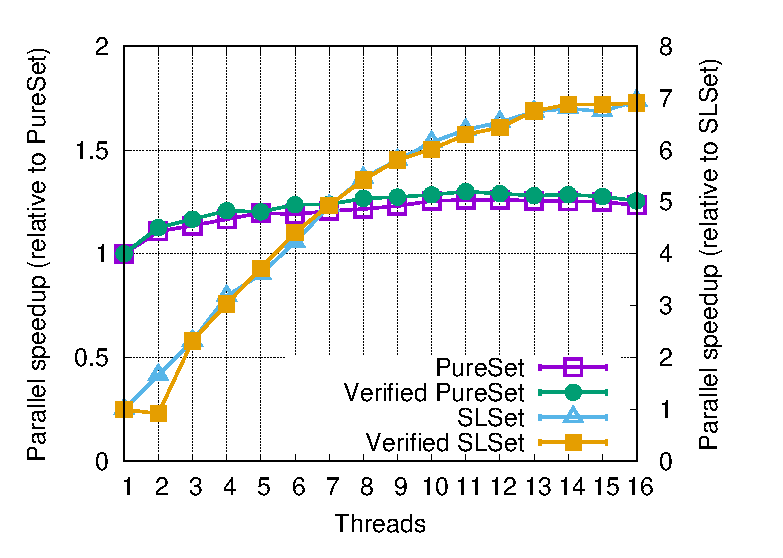
\includegraphics[width=3.2in]{text/refinementreflection/set.eps}
  \end{center}
  \caption[Parallel speedup for PureSet and SLSet.]
    {Parallel speedup for doing 1 million parallel inserts over 10
    iterations, verified and unverified, relative to the unverified version,
    for PureSet and SLSet.}
  \label{fig:set}
\end{figure}

\subsection{Monad-par: $n$-body simulation}
\label{sec:nbody}
Next, we verify deterministic behavior of an
$n$-body simulation program that leverages @monad-par@, a Haskell library which
provides deterministic parallelism for pure code \cite{monad-par}.

Each simulated particle is represented by a
type @Body@ that stores its position, velocity and mass.
%
The function @accel@ computes the relative acceleration
between two bodies:
\begin{mcode}
  accel :: Body -> Body -> Accel
\end{mcode}
where @Accel@ represents the three-dimensional acceleration
\begin{mcode}
  data Accel = Accel Real Real Real
\end{mcode}
%
To compute the total acceleration
of a body @b@ we
(1) compute the relative acceleration between @b@
and each body of the system (@Vec Body@) and
(2) we add each acceleration component.
%
For efficiency, we use a parallel @mapReduce@ for the above
computation that
first \textit{maps} each vector body to get the acceleration relative to @b@
(@accel b@) and then adds each @Accel@ value by pointwise addition.
%
@mapReduce@ is only deterministic if the element is a @VerifiedMonoid@
from \S~\ref{sec:detpar}.
%%
%%To compute the velocity of each body in the simulation
%%we map reduce
%%
%%
%%An $n$-body simulation is used to model the behavior of particles in some system
%%in which forces are acting on the particles. The code which we verify is adapted
%%from an implementation of the all-pairs variant (a traditional, brute-force
%%approach) to $n$-body simulation from \cite{parallel-n-body}. The datatype which
%%we are verifying represents a particle:
%%
%%
\begin{mcode}
mapReduce :: VerifiedMonoid b 1=> (a1->b) 1-> Vec a 1-> b
\end{mcode}
%
To prove the determinism of an $n$-body simulation, we need to provide a
@VerifiedMonoid@ instance for @Accel@.
%
We can easily prove that (@Real@, @+@, @0.0@)
is a monoid.
%
By product proof composition, we get a verified monoid instance for
\begin{mcode}
  type Accel' = (Real, (Real, Real))
\end{mcode}
which is isomorphic to @Accel@ (\ie @Iso Accel' Accel@).

Figure~\ref{fig:nbody} shows the results of running two versions of the $n$-body
simulation with 2,048 bodies over 5 iterations, with and without verification,
using floating point doubles for \texttt{Real}\footnote{Floating point numbers
  notoriously violate associativity, but we use this approximation because
  Haskell does net yet have an implementation of {\em
    superaccumulators}~\cite{superaccumulation}.}. Notably, the two programs have almost
identical runtime performance.  This demonstrates that even when verifying code
that is run in a tight loop (like @accel@), we can expect that our programs
will not be slowed down by an unacceptable amount.

\begin{figure}
\captionsetup{justification=centering}
  \begin{center}
    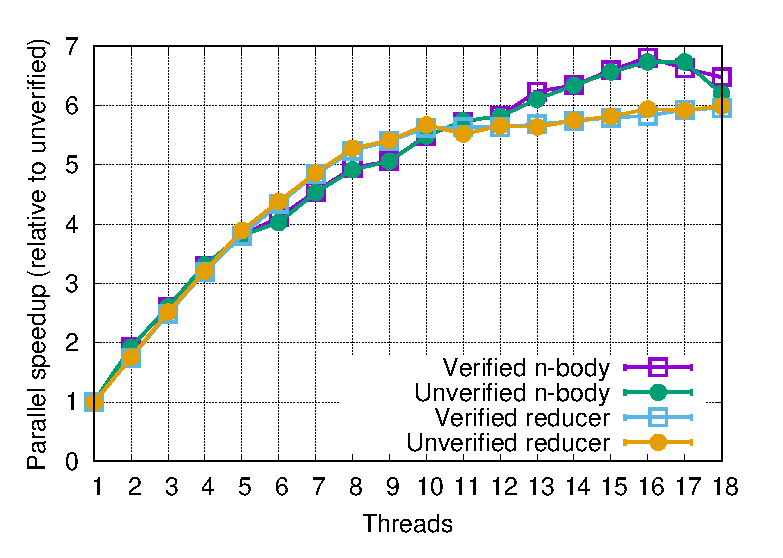
\includegraphics[width=3.2in]{text/refinementreflection/nbody.eps}
  \end{center}
  \caption[Parallel speedup for $n$-body simulation and array reduction.]
      {Parallel speedup for doing a parallel $n$-body simulation and
      parallel array reduction. The speedup is relative to the
    unverified version of each respective class of program.}
  \label{fig:nbody}
\end{figure}

\subsection{DPJ: Parallel Reducers}
\label{sec:reducer}
%% Our last benchmark illustrates how one can enforce various deterministic properties
%% that are different from the standard class properties (\ie monoid associativity).
%% For example,
The Deterministic Parallel Java (DPJ) project provides
a deterministic-by-default semantics for the Java programming language~\cite{DPJ}.
%
In DPJ, one can declare a method as @commutative@ and thus {\em assert} that
racing instances of that method result in a deterministic outcome.
For example:
%
% private region AccumRgn, static int sum in AccumRgn;
%% private static commutative synchronized
%%  void updateSum(int n) writes AccumRgn { sum += n; }
\begin{code}
commutative void updateSum(int n) writes R
  { sum += n; }
\end{code}
But, DPJ provides no means to formally prove commutativity and thus
determinism of parallel reduction.
In Liquid Haskell, we specified commutativity as an extra proof method
that extends the @VerifiedMonoid@ class.
%
\begin{mcode}
 class VerifiedMonoid a => VerifiedComMonoid a where
  commutes :: x:a -> y:a -> { x <> y = y <> x }
\end{mcode}
%
Provably commutative appends can be used to deterministically
update a reducer variable, since the result is the same regardless
of the order of appends.
%
We used LVish~\cite{kuper2014freeze} to
encode a reducer variable with a value @a@ and a region @s@
as @RVar s a@.
\begin{mcode}
 newtype RVar s a
\end{mcode}
We specify that safe (\ie deterministic)
parallel updates require provably commutative appending.
\begin{mcode}
  updateRVar :: VerifiedComMonoid a
             => a -> RVar s a -> Par s ()
\end{mcode}
%
Following the DPJ program, we used @updateRVar@'s provably deterministic interface
to compute, in parallel, the sum of an array with $3$x$10^9$ elements by updating
a single, global reduction variable using a varying number of threads.
%
Each thread sums segments of an array, sequentially, and updates the variable
with these partial sums.
%
In Figure \ref{fig:nbody}, we compare the verified and unverified versions
of our implementation to observe no appreciable
difference in performance.

